\chapter{ Аналитический раздел}
\label{cha:analysis}

\section{ Цвет}
С физической точки зрения цвет представляет собой свет, который, отражаясь от объекта, попадает в глаз человека. Восприятие цвета человеком может зависить от психологического состояния индивида, от местоположения объекта, от строение глаза человека, от окружаещего света и т.д. То есть восприятяие цвета человеком достаточно субъективно. Свет в свою очередь можно описать как волну, длинна которой возбуждает разные рецепторы человеческого глаза. То есть, индивид будет понимать какого цвета объект перед ним в зависимости от того, в какой диапазон попадет длинна волны света, отраженного от этого объекта.

\subsection{ Модели цвета}

Модель цвета -- абстрактная математическая модель представления цветов в виде кортежей чисел.

В какой-то момент необходимо было придумать модель цвета. Описать это явление так, чтобы можно было эффективно и удобно представлять цветовую информацию в цифровом виде. Проблема описания цвета в форме математики была решена еще до появления компьютеров. Одним из первых таких описаний было RGB(Red, green, blue) пространство, идея которого заключалась в представлении всех цветов, различимых человеком, с помощью трех базовых понятий - красного, зеленого и синего. RGB не является одним единственным пространством. Список основных цветовых пространств:
\begin{enumerate}
	\item RGB, sRGB, Adobe RGB
	\item CIEXYZ, CIELAB
	\item CMY(K)
	\item HSL, HSV
\end{enumerate}

$RGB$ -- пространство, строящееся на составление цвета из трех базовых -- красного(Red), синего(Blue) и зеленого(Green). Данную модель часто называют цветовым кубом, потому что каждый базовый параметр цвета, представленного в этой модели, может восприниматься как координата трехмерного пространства.

\begin{figure}[ht!]
	\centering{
		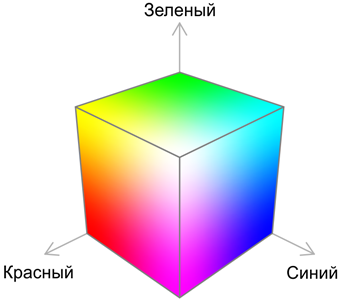
\includegraphics[width=0.4\textwidth]{img/colorCube.png}
		\caption{Представление цветового куба.}}
\end{figure}

Данная модель способна представить 16 777 216(\(2^8 * 2^8 * 2^8\)) цветов.\\

\textit{CIEXYZ(CIE - International Commission on Illumination)} -- модель, которая является экстраполяцией RGB модели. Данная модель охватывает все цвета, видимые человеком. Когда модель RGB расширили до видимых цветов появились отрицательные числа и чтобы избавиться от них были введены мнимые основные цвета X(мнимый красный), Y(мнимый зеленый), Z(мнимый синий).

\textit{CIELAB(L*a*b*)} -- цветовая модель, которая может отображать цвета за пределами, распознаваемыми человеком. Основывается на трех параметрах: L - яркости(Lightness) и двух цветовых каналов a и b. Проблема данного цветового пространства заключается в том, что расстояние между цветами в этой цветовой модели не соответствует цветовому спектру(Например, расстояние от зеленого к зелено-желтому большое в то время как от красного к синиму достаточно маленькое)

\begin{figure}[ht!]
	\centering{
		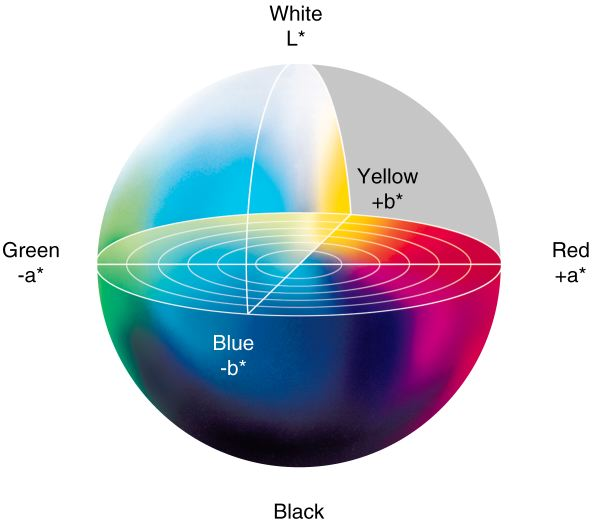
\includegraphics[width=0.4\textwidth]{img/lab.png}
		\caption{Представление цветовой модели CIALAB.}}
\end{figure}

\textit{CMY(K)} -- цветовая модель, аббревиатуру которой можно расшифровать как Cyan(голубой), Magenta(пурпурный), Yellow(желтый), blacK(Key). Данная цветовая модель широко используется в печати документов, изображений. Изначально в данном пространстве исплользовалось только три цвета: cyan, magenta, yellow, с помощью которых можно было получить и черный цвет, смешивая краски. Но это оказалось не эффективно и затратно, поэтому для черного решили ввести отдельный канал, что позволило сэкономить очень много средств.

\begin{figure}[ht!]
	\centering{
		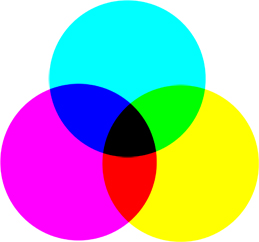
\includegraphics[width=0.4\textwidth]{img/cmyk.png}
		\caption{Представление цветовой модели CMYK.}}
\end{figure}\\

\textit{YUV, YIQ} -- цветовые модели, где информация о цвете передавалась в виде яркости(Y) и двху цветоразностных сигналов IQ/UV. Благодаря тому, что в Y изображение хранилось в градациях серого, изображение могло подаваться и на старые бесцветные телевизоры.\\

\textit{HSL, HSV} -- цветовые пространства, строящиеся на оттенке(Hue), насещенности(Saturation), яркости(Lightness) или значении(Value).

Яркость(L) и значение(V) -- это разные вещи:\\

\(R, G, B \in [0, 1]\)

\(V = \max{R, G, B}\)

\(L = \frac{1}{2} (\max{R, G, B} + \min{R, G, B})\)\\

Насыщенность у этих моделей тоже разная:\\

S_{HSV} = \frac{\max{R, G, B} - min{R, G, B}}{V}

S_{HSL} = \frac{\max{R, G, B} - min{R, G, B}}{1-|2L-1|}

\begin{figure}[ht!]
	\centering{
		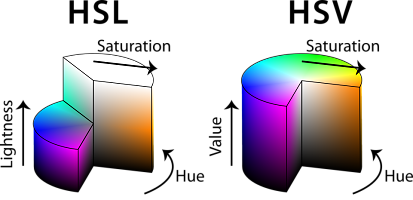
\includegraphics[width=0.4\textwidth]{img/hsl_hsv.png}
		\caption{Представление цветовой модели CIALAB.}}
\end{figure}

\subsection{ Пребладающий цвет}
Стоит выделить понятие преобладающий цвет, которое так часто использовалось выше. Цвет может быть преобладающим чисто математически/физически, а может быть преобладающим с точки зрения человека. Изображение, которое на 70\% состоит из черного цвета и на 30\% из оранжевого вносит неопределенность в выборе доминантного цвета. В первом случае преобладающий цвет рассматривается как нечто физическое. В таком случае доминирующий цвет - черный, потому что он занимает большую часть картники. Во втором преобладает оранжевый, т.к с точки зрения человека, глаз в первую очередь обратит внимание на более яркую, выразительную точку, чем темную и тусклую.
\subsection{ Квантование цвета}
Квантование -- разбиение диапазона значений некоторой величины на конечное число уровней и округление этих значений до ближайших к ним уровней.

Квантование цвета в изображении очень важная задача в компьютерной графике. Она позваляет уменьшить количество цветов отображаемой картинки. Это активно используется при сжатии, позволяя уменьшить глубину цвета, при добавлении эффектов на изображение. Следующие алгоримы позволяют решить данную задачу:
\begin{enumerate}
	\item Алгоритм равномерного(однородного) квантования.
	\item Алгоритм квантования цветов медианным сечением.
	\item Алгоритмы кластеризации(Например алгоритм k-средних).
\end{enumerate}

\textit{Алгоритм квантования цветов медианным сечением:}

Данный метод заключается в разбиении цветового пространства на параллелепипеды со сторонами, параллельными осям цветового пространства RGB.

Первый шаг заключается в нахождении минимального параллелепипеда, который содержит все цвета, представленые в изображении.

На втором шаге происходит определение самой длинной стороны параллелепипеда и сортировка всех значений вдоль выбранного направления. Далее параллелепипед разделяется по медиане множества значений выбранного направления на две части. Отсюда, получится два параллелепипеда, которые содержат примерно одинаковое количество значений. 

Предыдущая процедура повторяется до тех пор, пока не будет получено N параллелепипедов, где N - количество цветов новой палитры. После этого требуется заполнить палитру цветов, которая будет описывать изображение. Для каждого параллелепипеда нужно рассчитать цвет, который будет представлять его(либо центральная точка параллелепипеда, либо среднее арифметическое значение точек, попавших в него)

На самом изображении остается проанализировать пиксель(найти параллелепипед, в который попадает данная точка) и заменить цвет пикселя на цвет, который представляет весь параллелепипед.

\textit{Алгоритм кластеризации k-средних:}

Метод кластеризации основан на центроидах -- точках, которые представляют собой центр кластера.

Первый шаг алгоритма заключается в инициализации центроидов, количество которых равно N(размер требуемой палитры). Инициализация центроидов очень важный момент, который сильно влияет на работу всего алгоритма. Можно взять случайные центроиды, но это возможно приведет к погрешности.

Далее выделяется два основных шага данного алгоритма: нахождение кластеров, которые определяются путем кратчайшего расстояние от точки до центроида, и рассчитывание центра масс получившихся кластеров, смещение центроидов на полученные центры масс. Эти два шага повторяются до тех пор, пока центроиды не стабилизируются и больше не будут смещаться.

\begin{figure}[ht!]
	\centering{
		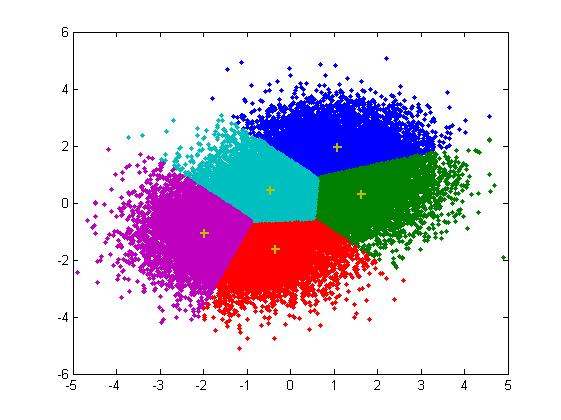
\includegraphics[width=0.4\textwidth]{img/k-means.jpg}
		\caption{Результат работы k-means с представленными центроидами.}}
\end{figure}

\subsection{ Цветовые гистограммы}
Гистограмма -- график статического распределения цифрового изображения с различной яркостью, в котором по горизонтальной оси представлена яркость, а по вертикали -- относительное число пикселей с конкретным значением яркости. С помощью гистограммы определяется насыщенность изображения(либо сумарная, либо разделенная по цветовым каналам).

\begin{figure}[ht!]
	\centering{
		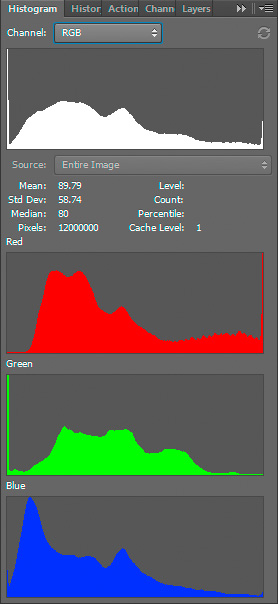
\includegraphics[width=0.4\textwidth]{img/histograms.jpg}
		\caption{Гистограммы, характеризующие изображение в программе Photoshop CS6.}}
\end{figure}

\subsection{ MPEG-7}
MPEG-7 -- стандарт ISO/IEC, разработанный группой MPEG(Moving Picture Experts Group). Аббревиатура расшифровывается как Multimedia Content Description Interface(Мультимедиа-интерфейс для описания содержимого). Имеет цель стандартизировать и описать мультимедийное пространство.

Стандарт состоит из семи частей:
\begin{enumerate}
	\item Системы MPEG-7.
	\item Язык описания определений MPEG-7.
	\item Audio -- дескрипторы и схемы описания аудио материала.
	\item Visual -- дескрипторы и схемы описания визуального материала.
	\item Multimedia Descriptor Schemes -- дескрипторы и схемы описания общих характеристик описания мультимедиа.
	\item Reference Software -- програмные реализации соответствующих частей стандарта.
	\item Conformance -- базовые принципы и процедуры тестирования рабочих характеристик практических реализаций стандарта.
\end{enumerate}

\subsection{ Трехмерное представление цвета}

\section{ Алгоритмы выделения преобладающего цвета}
\subsection{ Histogram algorithms}
\subsection{ GLA(generalized Lloyd Algorithm)}
\subsection{ Clustering algorithms}

\section{ Выбор подходящего алгоритма для решения задачи}
